\section{Methods}  \label{Methods}

In this section We propose a novel RNN architecture called the Recurrent Perceiver to model an object's changing appearance and motion over time for video object detection.
This section outlines the procedure used for training the models presented in this thesis.


\subsection{Model} \label{Methods:Model}

We build our model architecture based on the Perceiver architecture \cite{jaeglePerceiverGeneralPerception2021}. As discussed in \ref{Background:Perceiver} perceiver has capability of processing high dimantional input which is important for ADS. However, has a limitation of producing only one output per input, which makes it not approapriate for video object detection tasks. To overcome this limitation, we decided to rethink the Perceiver architecture and think of it as a recurrent neural network (RNN) that is capable to process a high dimentional input potentially from different modalities. Hence we have designed a Recurrent Perceiver or RPerciever for short. We have unrolled preceiver in time or in other words we have added a time dinemtion. If previously, the Perceiver was unrolled in depth, we closed the loop and unrolled it in time by propagating the latent array between time steps. For the initial timestamp we still use learnable latent array, the same way it is done in the Perceiver \ref{Background:Perceiver}. The architecture of the perceiver is Figure \ref{fig:figure_methods_recurrent_perceiver}.

% TODO add information about dimentions

% TODO edit fiture and name

\begin{figure}
    \centering
    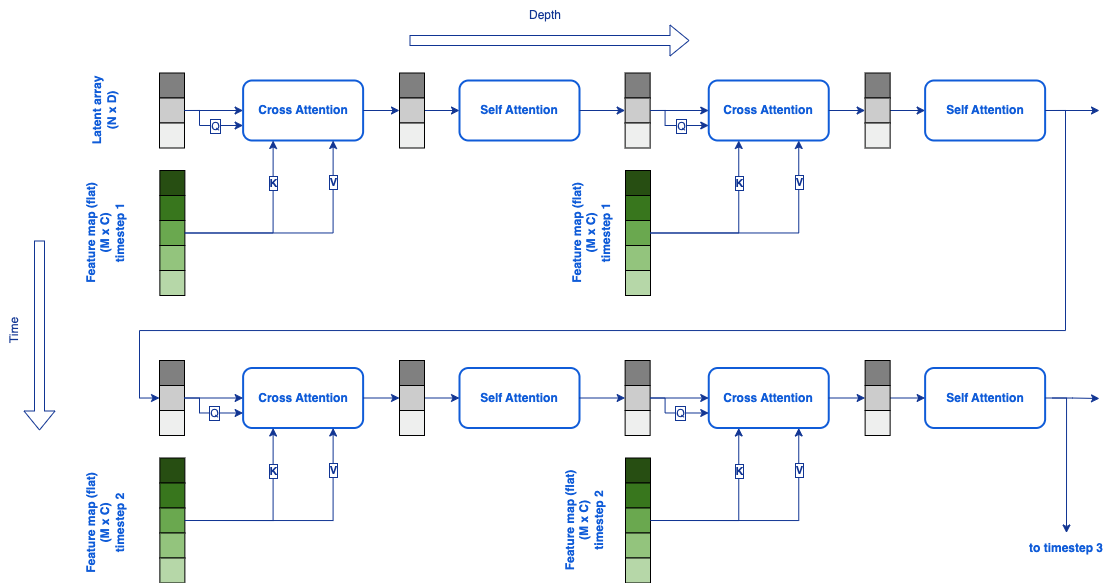
\includegraphics[width=\textwidth]{figures/figure_methods_recurrent_perceiver.png}
    \caption{The Recurrent Perceiver uses a conventional CNN backbone to learn a 2D representation of an input frame. The model flattens it and supplements it with a positional encoding before passing it to the autoregressive Perceiver model. Additionally, the autoregressive Perceiver takes a hidden state from the previous frame. We pass each output embedding of the Perceiver to the feed-forward network (FFN) that predicts class labels and center points.}
    \label{fig:figure_methods_recurrent_perceiver}
\end{figure}

We designed a variation of the RPerceiver to process multi-modal input. We call this arcitecture as Recurrent Perceiver Multi-Modal or RPerceiverMM for short. Modern ADS process information from multiple sensors. In the scope of the thesis, we consider a multi-view camera setup. \cite{jaeglePerceiverGeneralPerception2021} consider a multi-modality input where modality specific by concatenating a learned, modality-specific encoding to each input. In our work we followed a different approach for multi-modality. ADS is equiped with multiple cameras that are placed in different locations. There's exists a problem of calibrating. Therefore we decided to intorduce a camera specific cross-attention module to the RPerceiverMM. The architecture of the RPerceiverMM is shown on Figure~\ref{fig:figure_methods_model_ar_perceiver_views}.

% TODO edit fiture and name

\begin{figure}
    \centering
    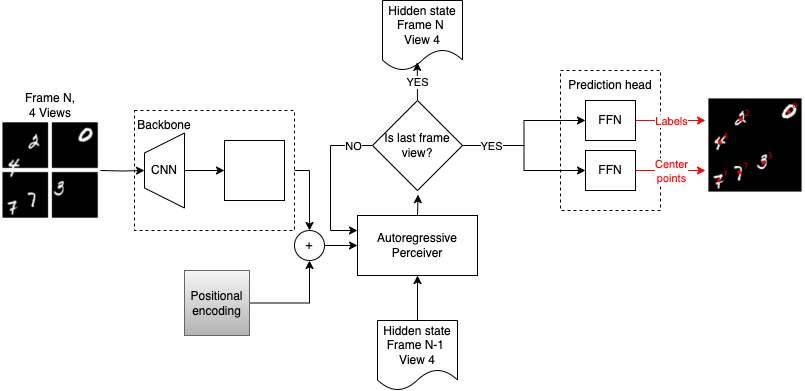
\includegraphics[width=\textwidth]{figures/figure_methods_model_ar_perceiver_views.png}
    \caption{Autoregressive Perceiver with view dimension. The backbone output is supplemented with a learned view-specific positional encoding before passing it to the autoregressive Perceiver model. The autoregressive Perceiver takes a hidden state from the previous frame's last view and iterates through the current frame's views. After the last view, we pass the output embedding of the Perceiver to the feed-forward network (FFN) that predicts class labels and center points on the global frame raster.}
    \label{fig:figure_methods_model_ar_perceiver_views}
\end{figure}

Additionally, to the Recurrent Perceiver (including Multi-modal variant), we used a CNN backbone to learn a 2D representation of the input frames, we did not use a pre-trained backbone see Appendix \ref{Appendix:Backbone}. We used a detection heads similar as in DETR model \cite{} with linear layer to project class logits and 3 layer of multi-layer perceptron (MLP) to predict the object coordinates. As for objects coordinates we considered two variants: (i) bounding boxes (ii) center point. Therefore the dimention of output $Lx4$ and $Lx2$ respectively. For bounding boxes we used a sigmoid activateion function to predict coordinates of bounding box center and width and hight. For center points we used a tanh activation function because we placed the center of the coordnate system into the center in order to mimic a berd-eye view, similar as ADS in center with all views around it. The whole and complete architecture is show \ref{fig:figure_methods_model_r_perceiver_complte}.

\begin{figure}
    \centering
    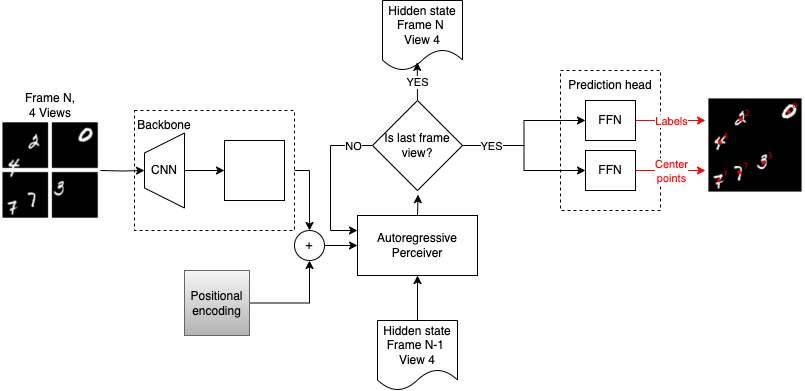
\includegraphics[width=\textwidth]{figures/figure_methods_model_ar_perceiver_views.png}
    \caption{Full architecture of our model. The backbone output is supplemented with a learned view-specific positional encoding before passing it to the autoregressive Perceiver model. The autoregressive Perceiver takes a hidden state from the previous frame's last view and iterates through the current frame's views. After the last view, we pass the output embedding of the Perceiver to the feed-forward network (FFN) that predicts class labels and center points on the global frame raster.}
    \label{fig:figure_methods_model_r_perceiver_complte}
\end{figure}


\subsection{Dataset} \label{Methods:Dataset}

For our experiment, we generated our own dataset, which we call "detection-moving-mnist-easy". We took inspiration from the MovingMNIST dataset \cite{srivastava2016unsupervisedlearningvideorepresentations}, which is used for TODO use cases. In our case, we are interested in video object detection and a simplified variation of keypoints, where we predict a center point of the object it is similar to keypoints task because the center of object is not the same as center of the bounding box. We hosted the dataset on Hugging Face \footnote{\url{https://huggingface.co/datasets/Max-Ploter/detection-moving-mnist-easy}}.

 For the first frame, we pick a number of digits from 1 to 10 with uniform probability (see Figure~\ref{fig:figure_method_dataset_train_digit_classes}). Depending on the number of digits per first frame, we draw, without replacement, from the well-known MNIST dataset \cite{} (from the train and test splits corresponding to the dataset split). Each digit is placed on the first frame of the canvas image of size 128x128. There's a greedy algorithm that places digits on the first frame randomly and tries to avoid overlaps, so it's easier for the model to detect all objects in the beginning. To each digit, we assign an affine translation from -5 to 5 randomly with uniform probability. Then, we apply corresponding affine transformations to move the digits through 20 frames on the canvas image of size 128x128. As a result, we receive a tensor of size 20x1x128x128, which represents a video (see Figure~\ref{fig:figure_methods_dataset_detection_mmnist_sequence}).

\begin{figure}
    \centering
    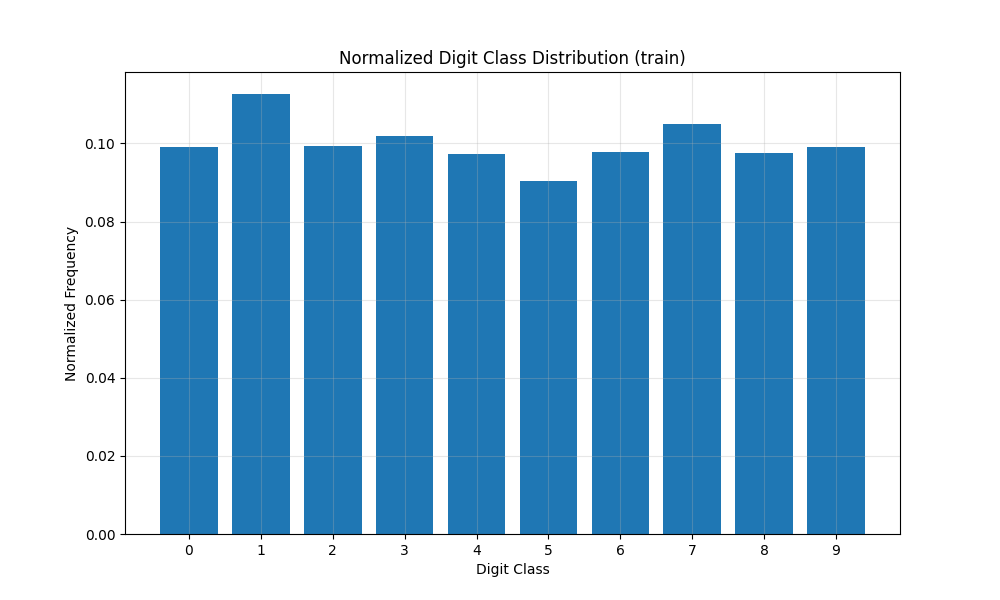
\includegraphics[width=\textwidth]{figures/figure_method_dataset_train_digit_classes.png}
    \caption{Distribution of classes in the "detection-moving-mnist-easy" dataset.}
    \label{fig:figure_method_dataset_train_digit_classes}
\end{figure}


\begin{figure}
    \centering
    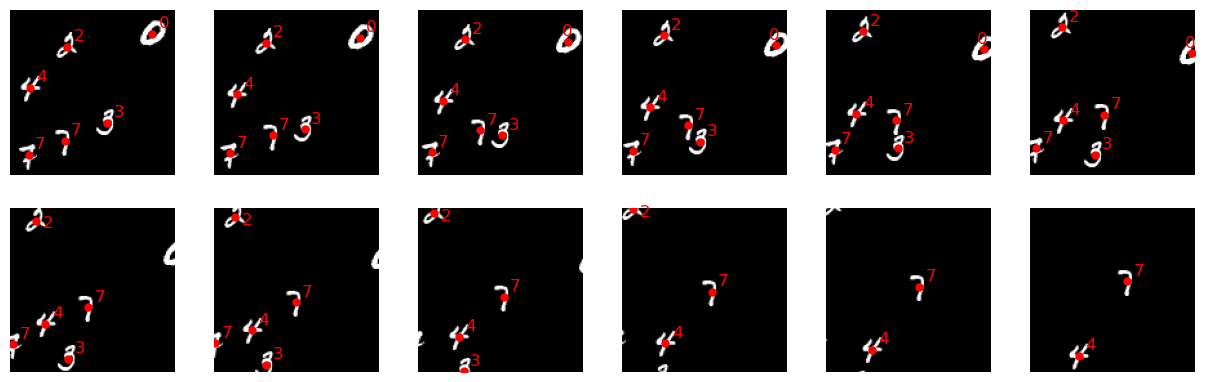
\includegraphics[width=\textwidth]{figures/figure_methods_dataset_detection_mmnist_sequence.png}
    \caption{Example of 12 frames from the sequence. Ground truth, shown in red, indicates the ground truth digit center point and a class label.}
    \label{fig:figure_methods_dataset_detection_mmnist_sequence}
\end{figure}


In order for dataset to be more challanging we do not restrict digit overlap in subsequent frames. It is even possible to have some degree of overlap in the first frame if the greedy algorithm is unable to randomly place digits in such a way on the first frame. We do not bounce digits against image boundaries, so each digit can leave the frame. You can see in the figure that later frames have fewer digits (see Figure~\ref{fig:figure_method_dataset_train_digits_per_frame}).

% TODO DOUBLE CHECK number this plot
\begin{figure}
    \centering
    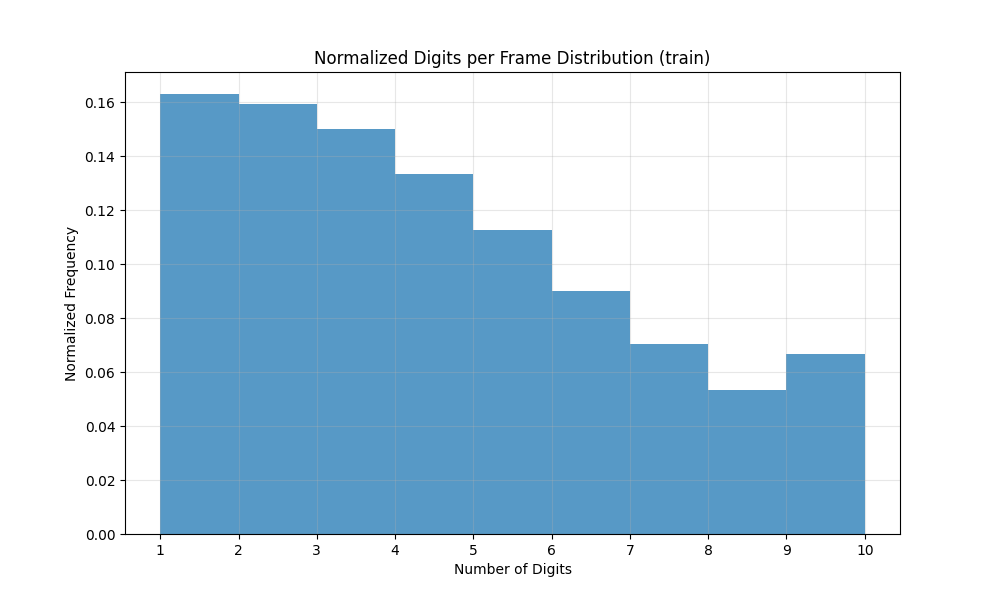
\includegraphics[width=\textwidth]{figures/figure_method_dataset_train_digits_per_frame.png}
    \caption{Distribution of classes in the "detection-moving-mnist-easy" dataset.}
    \label{fig:figure_method_dataset_train_digits_per_frame}
\end{figure}

We generated the dataset with 60K and 10K train and test splits, respectively. Annotations, automatically generated during sequence creation, include digit classes and digit center point coordinates (keypoint), bounding box coordinates and digit's identity ID.

\subsection{Metrics} \label{Methods:Metrics}

% TODO: mention mAP 75

We used mean Average Precision (mAP) as the primary metric to evaluate the model's performance. A widely used metric in object detection, mAP measures the average precision across various Intersection over Union (IoU) thresholds, adapted from information retrieval evaluation methods and popularized in challenges like PASCAL VOC \cite{everinghamPascalVisualObject2010}. Specifically, we report the mAP at an IoU threshold of 0.5, a common choice established in early object detection benchmarks such as PASCAL VOC \cite{everinghamPascalVisualObject2010}, and the mAP at 0.5-0.95, which represents the mean of the average precision calculated at IoU thresholds ranging from 0.5 to 0.95 with a step of 0.05, as introduced by the COCO challenge \cite{linMicrosoftCOCOCommon2015a}.

We used the Average Displacement Error (ADE) and Final Displacement Error (FDE) metrics to evaluate the model's performance. The ADE measures the average distance between the predicted and ground truth center points over the sequence of frames \ref{eq:ade}.

\begin{equation}
    \text{ADE} = \frac{1}{N \cdot T} \sum_{i=1}^{N} \sum_{t=1}^{T} || \hat{y}_{i,t} - y_{i,t} ||_2
    \label{eq:ade}
\end{equation}

The FDE measures the distance between the predicted and ground truth center points at the last frame of the sequence \ref{eq:fde}.

\begin{equation}
    \text{FDE} = \frac{1}{N} \sum_{i=1}^{N} || \hat{y}_{i,T} - y_{i,T} ||_2
    \label{eq:fde}
\end{equation}

\subsection{Loss Function} \label{Methods:LossFunction}

The model predicts \ref{Methods:Model} a fixed-size set of $N$ potential object detections, $ \hat{y} = \{\hat{y}_j\}_{j=1}^N $, in a single pass, where $N$ is chosen to be larger than the maximal number of actual objects in the frame. A core challenge lies in comparing this fixed-size prediction set $ \hat{y} $ to the variable-size ground truth set of objects, $ y = \{y_i\}_{i=1}^M $. The loss function addresses this by first finding an optimal bipartite matching between predictions and ground truth objects, and then calculating a loss that penalizes both incorrect matches and unmatched predictions assigned to a background class.

To establish the best possible one-to-one correspondence between the $N$ predictions and the $M$ ground truth objects ($M \le N$), we formulate a bipartite matching problem. We seek a permutation $ \hat{\sigma} $ of the prediction indices $ \{1, ..., N\} $ that minimizes the total matching cost between the first $M$ permuted predictions and the $M$ ground truth objects:
\begin{equation}
    \hat{\sigma} = \underset{\sigma \in \mathcal{S}_N}{\arg\min} \sum_{i=1}^M \mathcal{L}_{match}(\hat{y}_{\sigma(i)}, y_i)
    \label{eq:matching_argmin}
\end{equation}
where $ \mathcal{L}_{match}(\hat{y}_{\sigma(i)}, y_i) $ is the cost of matching prediction $ \hat{y}_{\sigma(i)} $ with ground truth object $ y_i $, and $ \mathcal{S}_N $ is the set of all permutations of $ \{1, ..., N\} $. This optimal assignment $ \hat{\sigma} $ is found efficiently using the Hungarian algorithm. Predictions $ \hat{y}_{\sigma(i)} $ for $ i > M $ (if any) and those predictions $ \hat{y}_{\sigma(i)} $ for $ i \le M $ that are not part of the optimal one-to-one matching found by the algorithm (due to the cost minimization potentially leaving some ground truth objects unmatched if all potential prediction matches are too costly) are considered unmatched and assigned to the background class.

Each ground truth object $ y_i $ is represented as $ (c_i, b_i) $, where $ c_i $ is the target class label and $ b_i \in [0, 1]^4 $ is a vector defining the normalized ground truth box center coordinates, height, and width. For a prediction $ \hat{y}_j $, we have the predicted class logits leading to probabilities $ \hat{p}_j(c) $ for all classes $ c $, and the predicted bounding box $ \hat{b}_j $.

Based on the provided code (`BoxHungarianMatcher`), the matching cost $ \mathcal{L}_{match}(\hat{y}_j, y_i) $ between prediction $ j $ and ground truth $ i $ is a weighted sum of costs considering class prediction and box similarity:
\begin{equation}
    \mathcal{L}_{match}(\hat{y}_j, y_i) = \lambda_{class} \mathcal{C}_{class}(c_i, \hat{p}_j) + \lambda_{bbox} \mathcal{C}_{L1}(b_i, \hat{b}_j) + \lambda_{giou} \mathcal{C}_{giou}(b_i, \hat{b}_j)
    \label{eq:match_cost_revised}
\end{equation}
The terms $ \lambda_{class}, \lambda_{bbox}, \lambda_{giou} $ correspond to the weights `cost_class`, `cost_bbox`, and `cost_giou` specified in the code's matcher configuration.
\begin{itemize}
    \item $ \mathcal{C}_{class}(c_i, \hat{p}_j) $ is the classification cost. The code implements two variants:
        \begin{itemize}
            \item If Focal Loss (`focal_loss=True`) is used for matching, this cost is derived from the Focal Loss formulation using predicted sigmoid probabilities for class $c_i$.
            \item Otherwise, it approximates the negative log-likelihood using $ -\hat{p}_j(c_i) $, where $ \hat{p}_j(c_i) $ is the softmax probability assigned by prediction $j$ to the ground truth class $ c_i $.
        \end{itemize}
    \item $ \mathcal{C}_{L1}(b_i, \hat{b}_j) $ is the L1 distance between the predicted and ground truth boxes: $ \|b_i - \hat{b}_j\|_1 $.
    \item $ \mathcal{C}_{giou}(b_i, \hat{b}_j) $ is the Generalized IoU (GIoU) cost, calculated as $ 1 - \text{GIoU}(b_i, \hat{b}_j) $.
\end{itemize}

After determining the optimal assignment $ \hat{\sigma} $ using the Hungarian algorithm, the total loss $ \mathcal{L}_{total} $ is calculated by summing loss contributions over all $N$ predictions. Let $ P $ denote the set of index pairs $ (j, i) $ such that prediction $ j = \hat{\sigma}(i) $ is matched to ground truth $ i $ in the optimal assignment. The loss for each prediction depends on whether it was matched.
\begin{equation}
    \mathcal{L}_{total}(y, \hat{y}) = \sum_{j=1}^N \mathcal{L}_j
    \label{eq:total_loss_revised}
\end{equation}
where $ \mathcal{L}_j $ is the loss for prediction $ \hat{y}_j $.

If prediction $ j $ is matched to ground truth $ i $ (i.e., $ (j, i) \in P $):
\begin{equation}
    \mathcal{L}_j = \mathcal{L}_{class}(c_i, \hat{p}_j) + \mathcal{L}_{box}(b_i, \hat{b}_j)
\end{equation}
If prediction $ j $ is unmatched (i.e., $ (j, i) \notin P $ for any $ i $):
\begin{equation}
    \mathcal{L}_j = \mathcal{L}_{class}(c_{\emptyset}, \hat{p}_j)
\end{equation}
Here, $ c_{\emptyset} $ represents the special "no object" or background class index (numerically `self.num_classes` in the code).

In practice, this is implemented by constructing a target classification tensor (`target_classes` in the code) of shape `(batch_size, N)`, initially filled with the $ c_{\emptyset} $ index. Then, for each matched pair $ (j, i) \in P $, the entry corresponding to prediction $ j $ in this tensor is updated with the actual ground truth class $ c_i $. The classification loss is then computed between the predicted logits and this target tensor.

The specific loss components, weighted according to the `weight_dict` parameter, are:
\begin{itemize}
    \item \textbf{Classification Loss ($ \mathcal{L}_{class} $):} Penalizes inaccuracies in class prediction.
        \begin{itemize}
            \item For matched predictions, the target is the ground truth class $ c_i $.
            \item For unmatched predictions, the target is the background class $ c_{\emptyset} $.
            \item Depending on the configuration (`focal_loss` parameter):
                \begin{itemize}
                    \item \textbf{Cross-Entropy Loss:} If `focal_loss=False`, standard cross-entropy loss is used (`loss_labels` function). The loss for the background class $ c_{\emptyset} $ is specifically down-weighted by the `eos_coef` parameter (applied via `empty_weight` tensor) to manage class imbalance.
                    \begin{equation}
                         \mathcal{L}_{class}(c, \hat{p}_j) = -\log \hat{p}_j(c) \quad (\text{weighted for } c=c_{\emptyset})
                    \end{equation}
                    \item \textbf{Focal Loss:} If `focal_loss=True`, the sigmoid-based Focal Loss (`loss_labels_focal` function using `sigmoid_focal_loss`) is employed, configured with parameters $ \alpha $ (`focal_alpha`) and $ \gamma $ (`focal_gamma`). This inherently handles class imbalance.
                    \begin{equation}
                         \mathcal{L}_{class}(c, \hat{p}_j) = \text{FocalLoss}(\hat{p}_j, c; \alpha, \gamma)
                    \end{equation}
                \end{itemize}
        The classification loss term is weighted by `weight_dict['loss_ce']`.

    \item \textbf{Bounding Box Loss ($ \mathcal{L}_{box} $):} This component applies *only* to matched pairs $ (j, i) \in P $. It is a linear combination of L1 loss and Generalized IoU (GIoU) loss (`loss_boxes` function):
    \begin{equation}
        \mathcal{L}_{box}(b_i, \hat{b}_j) = \lambda_{L1} \mathcal{L}_{L1}(b_i, \hat{b}_j) + \lambda_{giou} \mathcal{L}_{giou}(b_i, \hat{b}_j)
        \label{eq:box_loss_revised}
    \end{equation}
    where:
        \begin{itemize}
            \item $ \mathcal{L}_{L1}(b_i, \hat{b}_j) = \|b_i - \hat{b}_j\|_1 $ is the L1 norm. Weighted by $ \lambda_{L1} $ (`weight_dict['loss_bbox'] * bbox_loss_coef`).
            \item $ \mathcal{L}_{giou}(b_i, \hat{b}_j) = 1 - \text{GIoU}(box\_ops.box\_cxcywh\_to\_xyxy(b_i), box\_ops.box\_cxcywh\_to\_xyxy(\hat{b}_j)) $. Weighted by $ \lambda_{giou} $ (`weight_dict['loss_giou'] * giou_loss_coef`).
        \end{itemize}
        Both $ \mathcal{L}_{L1} $ and $ \mathcal{L}_{giou} $ components are normalized by the total number of actual ground truth boxes ($M$) across the batch (`num_boxes`).
\end{itemize}
This combined loss function guides the end-to-end training, encouraging the model to assign high confidence and accurate boxes to predictions matched with ground truth objects, while assigning low confidence (predicting the background class) to unmatched predictions.




% TODO double check the N variable
RPerceiver models infer a fixed-size set of $N$ predictions, in a single pass for the time step, where $N$ is set to be larger than the typical number of objects in an image. The main challange of training is to score predicted objects with respect to the ground truth. Our loss produces an optimal bipartite matching between predicted and ground truth objects, and then optimize object-specific (bounding box) losses.

The training objective was optimized using a composite loss function tailored to the specific task (object detection or center point prediction).

This criterion first employed a Hungarian matching algorithm (matcher) to assign predictions to ground truth targets based on a cost function considering class probabilities and spatial proximity (bounding box L1 distance, GIoU distance, or center point distance). Following the matching, specific loss components were calculated. For classification, either standard cross-entropy or Focal Loss (focal_loss=True) was used to address class imbalance, particularly weighting the 'no-object' class (eos_coef) and configured with α (focal_alpha) and γ (focal_gamma) parameters. For regression, depending on the task, losses included L1 loss for bounding box coordinates (loss_bbox, bbox_loss_coef), Generalized Intersection over Union (GIoU) loss (loss_giou, giou_loss_coef), or L1 loss for center point prediction (loss_center_point, weight_loss_center_point). The relative contribution of each loss component was controlled by specific weight coefficients (e.g., weight_dict).

\subsection{Dropout and Shuffle} \label{Methods:Training:DropoutAndShuffle}

We implemented two training procedures: \texttt{shuffle} and \texttt{dropout}. Additionally, we implemented a combination of the two. A model trained without applying these training procedures is considered the baseline.

\begin{description}
    \item[\texttt{shuffle}] In this procedure, the sensor inputs are randomly permuted within each time step. Consequently, the model receives inputs from the sensors in a random order for that specific time step. This shuffling only occurs for sensor inputs within the same time step. This training procedure is only applicable to a multi-view setup.

    \item[\texttt{dropout}] This procedure simulates scenarios where sensor information is missing. To achieve this, we train the model by intermittently dropping sensor inputs (input dropout). We keep the first half of the input sequence intact (no dropout), allowing the model to accumulate features in its hidden state. The second half of the sequence may undergo frame dropout depending on the dropout probability. During training, we gradually increase the probability of an information dropout from 10\% up to 86.6\%.
\end{description}


% TODO add schema of shuffle and dropout

% TASK DEFINITION
